\documentclass[11pt]{article}
\usepackage{geometry} % see geometry.pdf on how to lay out the page. There's lots.
\usepackage{hyperref}
\usepackage{graphicx}
\usepackage{gensymb}
\usepackage[affil-it]{authblk}
\usepackage[toc,page]{appendix}
\usepackage{pifont}
\usepackage{amsmath}
\usepackage{amssymb}
\usepackage{relsize}
\usepackage{draftwatermark}
\usepackage[mathscr]{eucal}
\usepackage{amsmath, amssymb, graphics, setspace}
\usepackage{amsthm}
\usepackage[english]{babel}
 
\newcommand{\mathsym}[1]{{}}
\newcommand{\unicode}[1]{{}}

\newtheorem{exercise}{Exercise}
\newtheorem{theorem}{Theorem}
\newtheorem{corollary}{Corollary}

\SetWatermarkText{DRAFT}
\SetWatermarkScale{6}
\SetWatermarkLightness{0.95}

\DeclareMathOperator{\atantwo}{atan2}
\DeclareMathOperator{\sign}{sign}
\DeclareMathOperator{\sense}{sense}

% \geometry{letter} % or letter or a5paper or ... etc
% \geometry{landscape} % rotated page geometry

% See the ``Article customise'' template for come common customisations

\title{Formulae for the Helix Formed by Stacking Similar Objects}
\author{Robert L. Read
  \thanks{read.robert@gmail.com}
}
\affil{Founder, Public Invention, an educational non-profit.}

\date{\today}

%%% BEGIN DOCUMENT
\begin{document}

\maketitle

%% \tableofcontents

\section{Introduction}

During the Public Invention Mathathon of 2018, software was created to view tetrahedra joined face-to-face in chains. It
was noted by the participants that when the rules for which face to add the next tetrahedron to were periodic, the resulting
chain was always a helix or a torus. A torus is a degenerate helix.

After some relfeciton, it became clear that any stack of objects of the same length joined at the same angles to each other repetitively form a helix. 
A specific example is a face-to-face connection of physical objects of the same length where the angles of the two joining
faces relative to each other control the angle and rotation of the axis at each joint. We have not yet found this simple idea articulated elsewhere. The purpose of this paper is to prove and to provide formulae for the resulting helix.

\section{A Warm-up: 2Dimensions}

Considering the problem in two dimensions may be a valuable introduction.
Suppose that we consider a polygon that that as two edges, called $A$ and $B$, and that we define the length $L$ of the
polygon as the distance between the midpoints of these edges. Suppose that we are only allowed to join these
polygons by aligning $A$ of one polygon to $B$ of another polygon, with their midpoints coincident. Let us
further assume that we disallow inversions of the polygon.  Let us imagine that we have a
countable number of polygons $P_i$ indexed from $0$. Then what shapes can we make by chaining these
polygons together?

Each joint $J_i$ between polygons $P_i$ and $P_{i+1}$ will place the axes of at the same angle, $\theta$, since
our polygons do not change shape. Let us define $\theta$ to be positive
if we move anti-clockwise from $P_i$ to $P_{i+1}$ and negative if we move clockwise. 
If $\theta = 0$, the joints will be collinear.

\begin{figure}
     \centering
     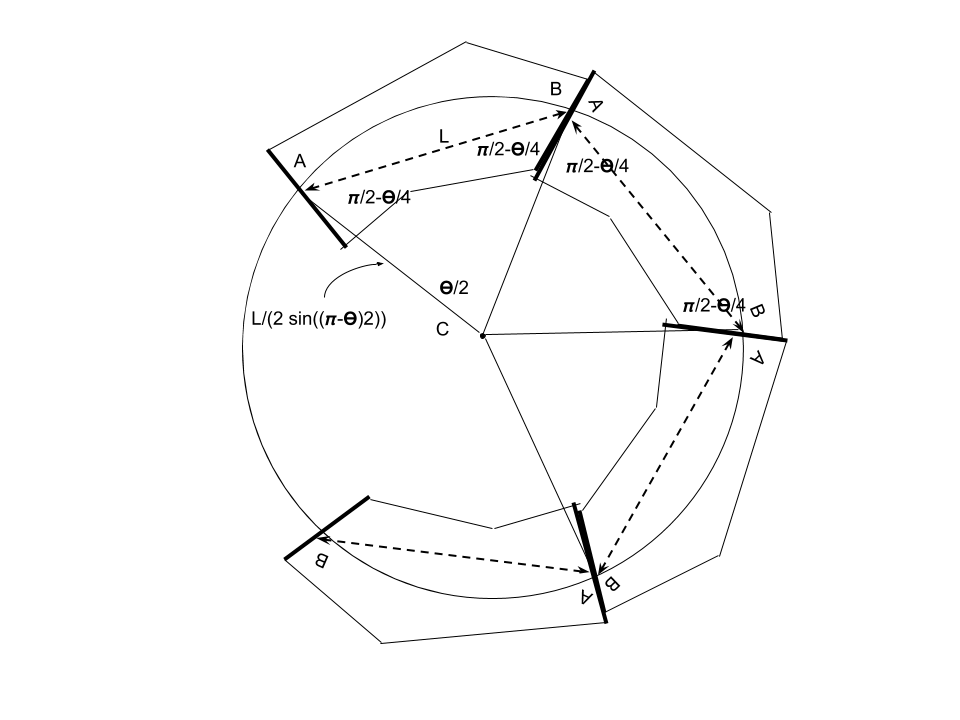
\includegraphics[width=0.80\textwidth]{figures/2DPolygonStacking.png}
     \caption{The rotatable prism of three objects}
  \label{fig:prismdiagram}
\end{figure}

If $\theta \neq 0$, it seems they polygon joints will always lie on a circle. A proof of this
is that each polygon has associated with it an isoceles triangle $A,B,C$, where $\angle CBA = \angle CAB = \theta/2$,
and $\angle ACB = (\pi - \theta)$. $AC$ and $BC$ are not necessarily aligned with an edge of the polygon.
The length $AB$ is $L$, and the lengths $AC$ and $BC$ are
$(L/2) / \sin{(\pi - \theta)/2}$. In any chain of polygons, these triangles all meet at point $C$, and there all
joints are on the circle centered at $C$ with radius $\frac{L}{2 \sin{\frac{\pi - \theta}{2}}$.

An analogous, though far more complicated, result holds in three dimensions.

\section{Three dimensions}


Consider a slender cylinder or prism with two faces $F_0,F_1$ cut at arbitrary angles to the axis of the cylinder.
Joining two such cylinders at the axes by placing $F_0$ angainst $F_1$ produced a joint with a difference in
angle between the axes of $\alpha$ and a rotation of the orienation of the faces about the axis of $\theta$.

\begin{theorem}[Stacking Helix]
  The joints of a sequential stack of objects of length $L$ whose joints axis change of $\alpha$ and orientation rotation
  of $\theta$ are intersected by a helix of radius.
\end{theorem}

\begin{figure}
     \centering
     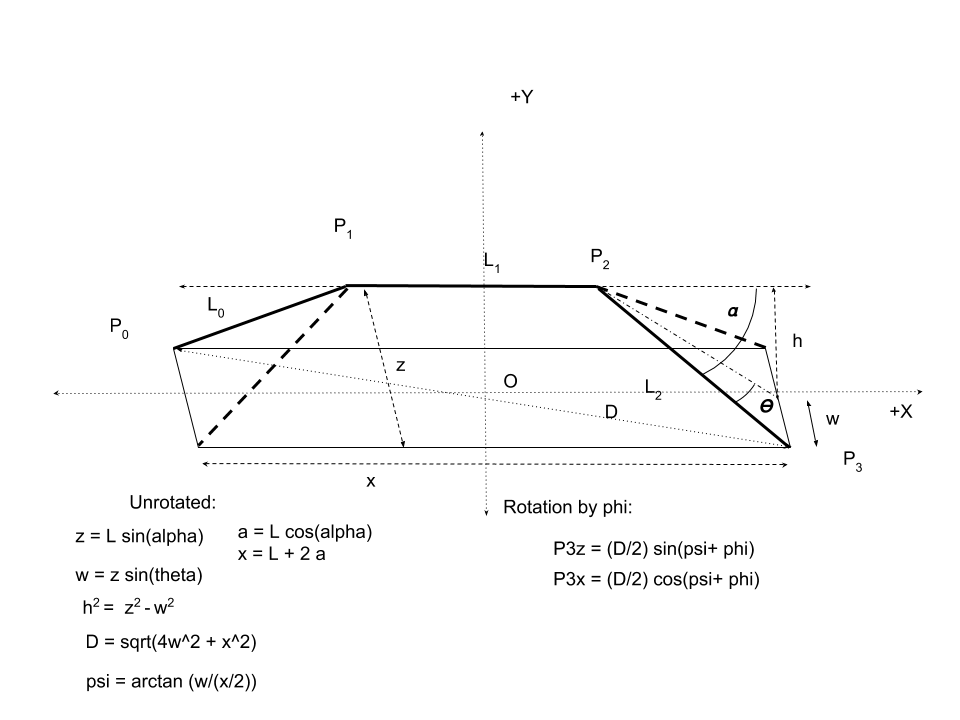
\includegraphics[width=0.80\textwidth]{figures/StackedSetup.png}
     \caption{The rotatable prism of three objects}
  \label{fig:prismdiagram}
\end{figure}

\begin{proof}

  In Figure \href{fig:prismdiagram}, let $L_i$ be the $i$th instance of the length-$L$ objects. Let $\alpha$ be the
  change in angle in the axes at a joint (the point were axes meet) measured in the plane containing the axes of both objects.
  Let $\theta$ be the change in orientation relative axis,
  or, the half-angle formed by $L_0$ and $L_2$ when projected onto a plane normal to the axis of $L_1$.
  Without loss of generality, choose the measures of these angles in radians so that
  $0 \leq \theta \pi/2$. Take $\alpha < 0$ to mean that objects $L_0$ and $L_1$ bend away from each other,
  and $\alpha > 0$ to mean that the objects $L_0$ and $L_1$ bend toward each other.
  If $\theta = 0$ and $\alpha > 0$, the stack will form a circle-like structure, where as if
  $\theta = 0$ and $\alpha < 0$, then stack will form a sawtooth-like structure.

  Note that any angle $\alpha$ is possible, if we do not concern oursleves with the self-collision
  of physical objects. $\alpha > \pi/2$ means the stack ``turns back on itself'' to some extent.

  If we arrange object $L_1$ so that its axis lies on the $x$-axis and its midpoint is at the origin,
  $L_0$ and $L_1$ extend from it symmetrically in the projection onto the $yz$-plane along the $x$-axis, which is always possible, and define $h$ to be the height of the faces of $L_0$ and $L_2$ along the $y$-axis
  and $w$ to be the distances between these faces in the $z$-dimesnion. Then we have:

  \begin{align*}
z &= L \sin{\alpha} \\
w &= z \sin{\theta} \\
h &= \sqrt{z^2 - w^2} \\
  \end{align*}

  Now we seek the formula for the helix which intersects the joints. To find the radius of this helix,
  we conceptually place our three objects in a cylinder, with the axis of $L_1$ along the surface
  of the cylinder aligned with the axis. We can size this cylinder to include the joints at the
  extreme ends of $L_2$ and $L_0$ as well. However, the $L_1$ axis lies on the surface, but
  the axes of $L_0$ and $L_2$ in general do not. If there exists a helix which intersects all
  joints, all axes will cut through this cylinder in the same way, creating chords in the projection
  into the $yz$-plane of the same length. Name these chords $c_0,c_1, and c_2$.

  Because we will need them later, we work out the geometry of this prism-like stack of three
  objects completely.
  \begin{itemize}
  \item The three objects are named $L_0,L_1,$ and $L_2$.
    $L_0$ has joints $P_0$ and $P_1$,
    $L_1$ has joints $P_1 and P_2$,
    $L_2$ has joints $P_2 and P_3$.
  \item  $x$ is the total length of the prism along the $x$-axis.
  \item $z$ is the length of the ``face'' of the prism, and the length
    of the chord before any rotation about $\phi$.
  \item $w$ is half of the width of the prism in the $z$-dimension.
  \item $h$ is the height of the prism in the $y$-dimension.
  \item $D$ is the length of the diagonal from $P_0$ to $P_3$.
  \item $\psi$ is the angle of $\overline{P_3O}$.
    \item $\phi$ is the amount we will have to rotate the prism about the $y$-axis.
    \end{itemize}
Given these defintions about our assumptions:
  \begin{align*}
c_0 &= z \cos{\phi} \\
c_1 &= L \sin{\phi} \\
c_2 &= z \cos{\phi} \\
D &= \sqrt{4w^2+x^2}
  \end{align*}
  

  We can imagine turing our 3-object stack and simulataneously increasing the size of our intersecting
  cyliner. If we turn the stack about the $y$-axis by $\phi$ degrees and keep the cylinder intersection
  the two faces of $L_1$, then the length of the $L_1$ chord will gradually increase. At the same time,
  the $L_0$ and $L_2$ chords will decrease. When $\phi = 0$, $c_0 = z, c_1 = 0, c_2 = z$.

  \begin{align*}
c_0 &= z \cos{\phi} \\
c_1 &= L \sin{\phi} \\
c_2 &= z \cos{\phi} \\
  \end{align*}
Equating these quantities:
    \begin{align*}
      z \cos{\phi}  &= L \sin{\phi} \\
      \frac{z}{L} &= \tan{\phi} \\
      \phi &= \arctan{\frac{z}{L}}  \\      
    \end{align*}
    Thus, by rotating our stack of objects $\phi$ degrees around the $y$-axis 
    all four faces of our three objects intersect a cylinder on its surface with
    equal rotational and axial distance. The axial distance between any two joints
    on the same object is $L \cos{\phi}$,
    and the length of the projected chord is $L \sin{\phi}$.

    The points $P_0,P_1,P_2,$ and $P_3$ now exist on a cylinder or unknown radius parallel
    to $x$-axis, and are evenly spaced along and evenly rotated about the axis of the
    cylinder. The joints points thus coincide with a general helix.

    Let us choose our coordinate system so that the $x$-axis corresponds to the
    axis of the helix. The general equation for the helix is:

\begin{align*}
    P_x(n) &= \kappa  t  \\
    P_y(n) &= r \cos{t} \\
   P_z(n) &= r \sin{t}
\end{align*}

We seek to discover $r$ and $\kappa$ based on our knowledge of $P_3$ and $P_2$.
In particular, we can deduce from the axial spacing there exists some $t_0$ such
that $P_2 = P(t_0)$ and $P_3 = P(3t_0)$.
Since we know that after rotation that:

  \begin{align*}
    P_{3z} &= (D/2) \sin{\phi + \psi} \\
    P_{3z} &= r\sin{3t_0} \\
    P_{2z} &= \sin{\phi} \\
    P_{2z} &= r\sin{t}
  \end{align*}
  We can use symbolic computation to solve this system of 2 equations and 2 unkowns:
  \begin{align*}
    r\sin{3t_0} &= (D/2) \sin{\phi + \psi} \\
    r\sin{t} &= \sin{\phi}
  \end{align*}
  Defining symbols:
  \begin{align*}
    E &= (D/2) \sin{\phi + \psi} \\
    F &= \sin{\phi}
  \end{align*}
  Wolfram alpha solves the system:
  \begin{align*}  
    r\sin{3t_0} &= E \\
    r\sin{t_0} &= F
  \end{align*}
  giving the result ($3F \neq E$ and $F \neq 0$), and ignoring multiples of $2\pi$ in $t$:

  
  \begin{align*}  
    r &= \frac{2F^{\frac{3}{2}}}{\sqrt{3F - E}} \\
    t_0 &= -2 \arctan{x}
      \frac{r +
        \sqrt{- \frac{F^2(F+E)}{E-3F}
        }
      }
           {F}
     \\
  \end{align*}
  From which, using $P_{2x} = L/2 = \kappa t_0$, we conclude:
  \begin{align*}  
    r &= \frac{2F^{\frac{3}{2}}}{\sqrt{3F - E}} \\
    \kappa &= \frac{L}{4 \arctan{\frac{r + \sqrt{- \frac{F^2(F+E)}{E-3F}}}{F}}}
  \end{align*}.
  Putting this all together we have:
  \begin{align*}
    a &= L \cos{\alpha} \\
    x &= L + 2a \\
    z &= L \sin{\alpha} \\
    w &= z \sin{\theta} \\
    h &= \sqrt{z^2 - w^2} \\
    D &= \sqrt{4w^2+x^2} \\
    \phi &= \arctan{\frac{z}{L}} \\
    E &= (D/2) \sin{\phi + \psi} \\
    F &= \sin{\phi} \\
    r &= \frac{2F^{\frac{3}{2}}}{\sqrt{3F - E}} \\
    \kappa &= \frac{L}{4 \arctan{\frac{r + \sqrt{- \frac{F^2(F+E)}{E-3F}}}{F}}}
  \end{align*}
  Using these values derived exclusively from the inputs $L,\alpha, and \theta$, we can
  evalute the formula for the general helix only and integral values of $n$ to
  obtian a formula for precise the joint points of this any such stack.
\begin{align*}
    P_x(n) &= \kappa  t0 (1 + 2n)  \\
    P_y(n) &= r \cos{t0 (1 + 2n)} \\
    P_z(n) &= r \sin{t0 (1 + 2n)}
\end{align*}

\end{proof}

\section{Checking against comprehensible values}

Unfortunately, the complexity of these formualae exceed the author's comprehension.
However, we may check these formuale by graphing them against comprehensible
examples. Obvious examples are extreme solutions, where $\alpha$  and $\theta$ are
$0$ or $\pi/2$, for example. We also have the particular non-trivial example
of the Boerdick-Coxeter tetrahelix, formed by regular tetrahedra, which has
been studied enough to have a known pitch.

\section{Implications}

One of the implcations of this is that it may be possible to design helixes
of any radius and pitch by designing periodic segments. Combined with slight
irregularites, this means that you have a basis of design molecular helices
out of ``atoms'' which correspond to our objects.


\section{Applied to Periodic Regular Simplex Chains}

\begin{corollary}
  Every regular simplex chain formed by a periodic generator has a helical structure.
  \end{corollary}

Prove or disprove that {\em every} periodic 3D Generator generates a figure contained within a cylinder of unbounded length but bounded diameter.

Note: Every example that we have tested exhibits this property. We believe it is a property of any repeated structure, not related to simplices.
However, we do not yet know the name of this theorem or principle. We conjecture that every stack of repeated truncated prisms
forms a helical aperigon, which is hinted at but not stated in the Wikipedia article\url{https://en.wikipedia.org/wiki/Skew_apeirogon}.

Note: Rob believes a proof that any periodic structure fits within a cylinder is possible, and that it should be possible to give a formulaic bound
on the diameter of this cylinder (under some assumptions.) The key to the proof is to use symmetry and focus on the the center of three
such objects, observing that the other two must necessarily bend towards or away from each other in a way describable by two angles.
A formula for the cylinder as a function of these angles would convincingly complete the proof.



\bibliographystyle{unsrt}
\bibliography{gluss}


\end{document}



